\documentclass[dvipdfmx,a4paper]{jsarticle}
\usepackage{amsmath,amssymb}
\usepackage{amsthm}
\usepackage{bm}
\usepackage[dvipdfmx]{graphicx}
\usepackage{ascmac}
\usepackage{subfigure}
\usepackage{verbatim}
\usepackage{wrapfig}
\usepackage{makeidx}
\usepackage[dvipdfmx]{hyperref}
\usepackage{setspace}
\usepackage{color}
\usepackage{listings}
\usepackage{cleveref}
\usepackage{mathtools}
\usepackage{framed}
\usepackage[textwidth=50zw,lines=46]{geometry}
\usepackage{here}
\usepackage{siunitx}

\usepackage{listings, jlisting, color}
\definecolor{OliveGreen}{rgb}{0.0,0.6,0.0}
\definecolor{Orenge}{rgb}{0.89,0.55,0}
\definecolor{SkyBlue}{rgb}{0.28, 0.28, 0.95}
\lstset{
  language={C++}, % 言語の指定
  basicstyle={\ttfamily},
  identifierstyle={\small},
  commentstyle={\smallitshape},
  keywordstyle={\small\bfseries},
  ndkeywordstyle={\small},
  stringstyle={\small\ttfamily},
  frame={tb},
  breaklines=true,
  columns=[l]{fullflexible},
  numbers=left,
  xrightmargin=0zw,
  xleftmargin=3zw,
  numberstyle={\scriptsize},
  stepnumber=1,
  numbersep=1zw,
  lineskip=-0.5ex,
  keywordstyle={\color{SkyBlue}},     %キーワード(int, ifなど)の書体指定
  commentstyle={\color{OliveGreen}},  %注釈の書体
  stringstyle=\color{Orenge}          %文字列
}

\begin{document}

\title{課題演習C3\quad 最終レポート}
\author{0500-34-0042\quad 大平 達也}
\date{2025/01/23}
\maketitle
\section{目的}
系外惑星TOI1516 bのTransit検出を目標とする。

\section{観測}
京都大学理学部4号館屋上の\SI{40}{cm}望遠鏡を用いて, ノンフィルターでの観測を行った。分かっている, 観測日におけるターゲットの情報は以下の通り:
\begin{description}
  \item[観測日] 2024/11/11
  \item[ingress] 20:00
  \item[degrees] 22:50
  \item[視等級] 10.8 mag
  \item[減光量] 0.016 mag
\end{description}
今回は, ingressの途中から観測を始めた。
\section{これまでの進捗状況}
\subsection{データの一次処理}
IRAFを用いて, 11/11に取得した観測データの一次処理を行った。
\subsection{測光用コードの開発}
途中までIRAFのスクリプトを書いていたが, 途中からPythonでの開発に切り替えた。作成したコードは以下の通り。なおアパーチャーの半径はHWHMの1.2倍とした。 

\subsection{測光結果}
相対測光により, TOI1516の等級を各画像で求めた。これをplotしたものを図\ref{fig:toi1516}に示す。

\begin{figure}[H]
  \centering
  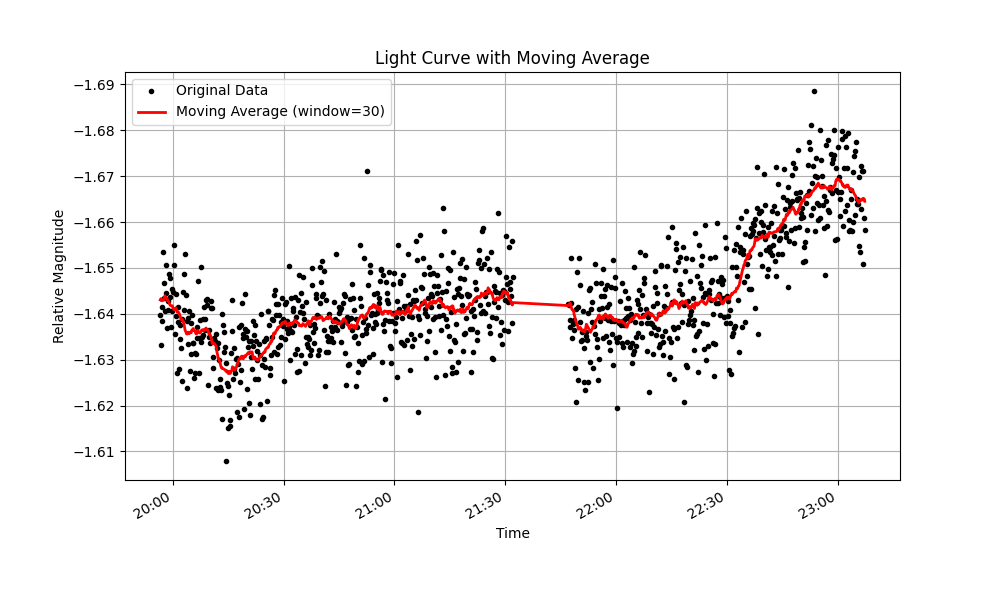
\includegraphics[width=0.9\textwidth]{./fig/light_curve_toi1516_with_moving_average.png}
  \caption{TOI1516の光度曲線}
  \label{fig:toi1516}
\end{figure}

\subsection{参照星の選び方について}
参照星は, 常に視野内に位置し, ターゲット星と同程度の明るさのものを選んだ。また, 測光したのちに, 参照星の等級の時間変化を調べ, 参照星として適切であるか検証した。

たとえば, 最初に選んだ参照星の等級の時間変化は図\ref{fig:comp}であった。全体として同じようなトレンドではあるが, Comp 4 (紫) のみノイズが大きいように見える。実際, Comp 4が参照星の中で最も暗い星であったことから, 参照星として選ぶのは適切でないと判断し, 他の参照星を選んだ。これを繰り返すことで, 最終的な参照星を選んだ。

なお, 参考までに, TOI1516の高度からエアマスを計算したplotも掲載しておく (図\ref{fig:airmass})。観測データから, 参照星の等級は時間とともに暗い方へ変化していったためエアマスには反する結果となった。原因は不明。

\begin{figure}[H]
  \centering
  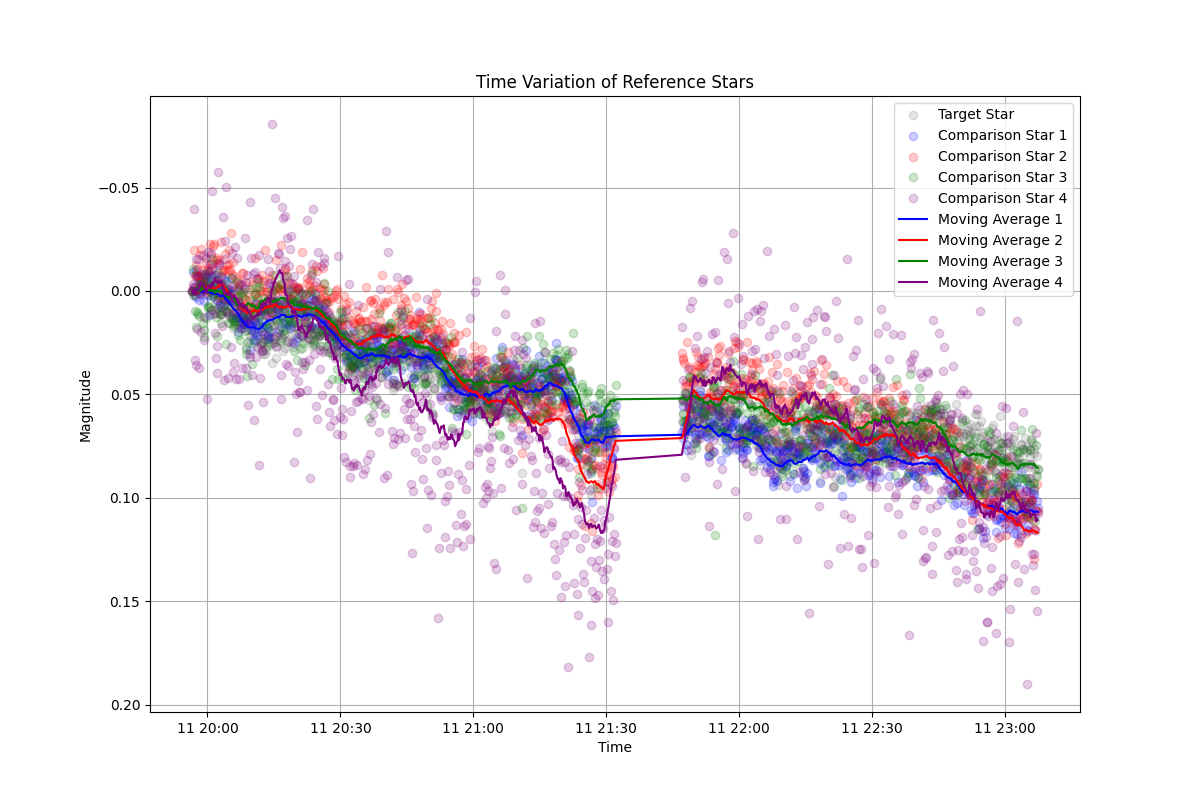
\includegraphics[width=0.9\textwidth]{./fig/light_curve_comp_first.png}
  \caption{参照星の光度曲線}
  \label{fig:comp}
\end{figure}

\begin{figure}[H]
  \centering
  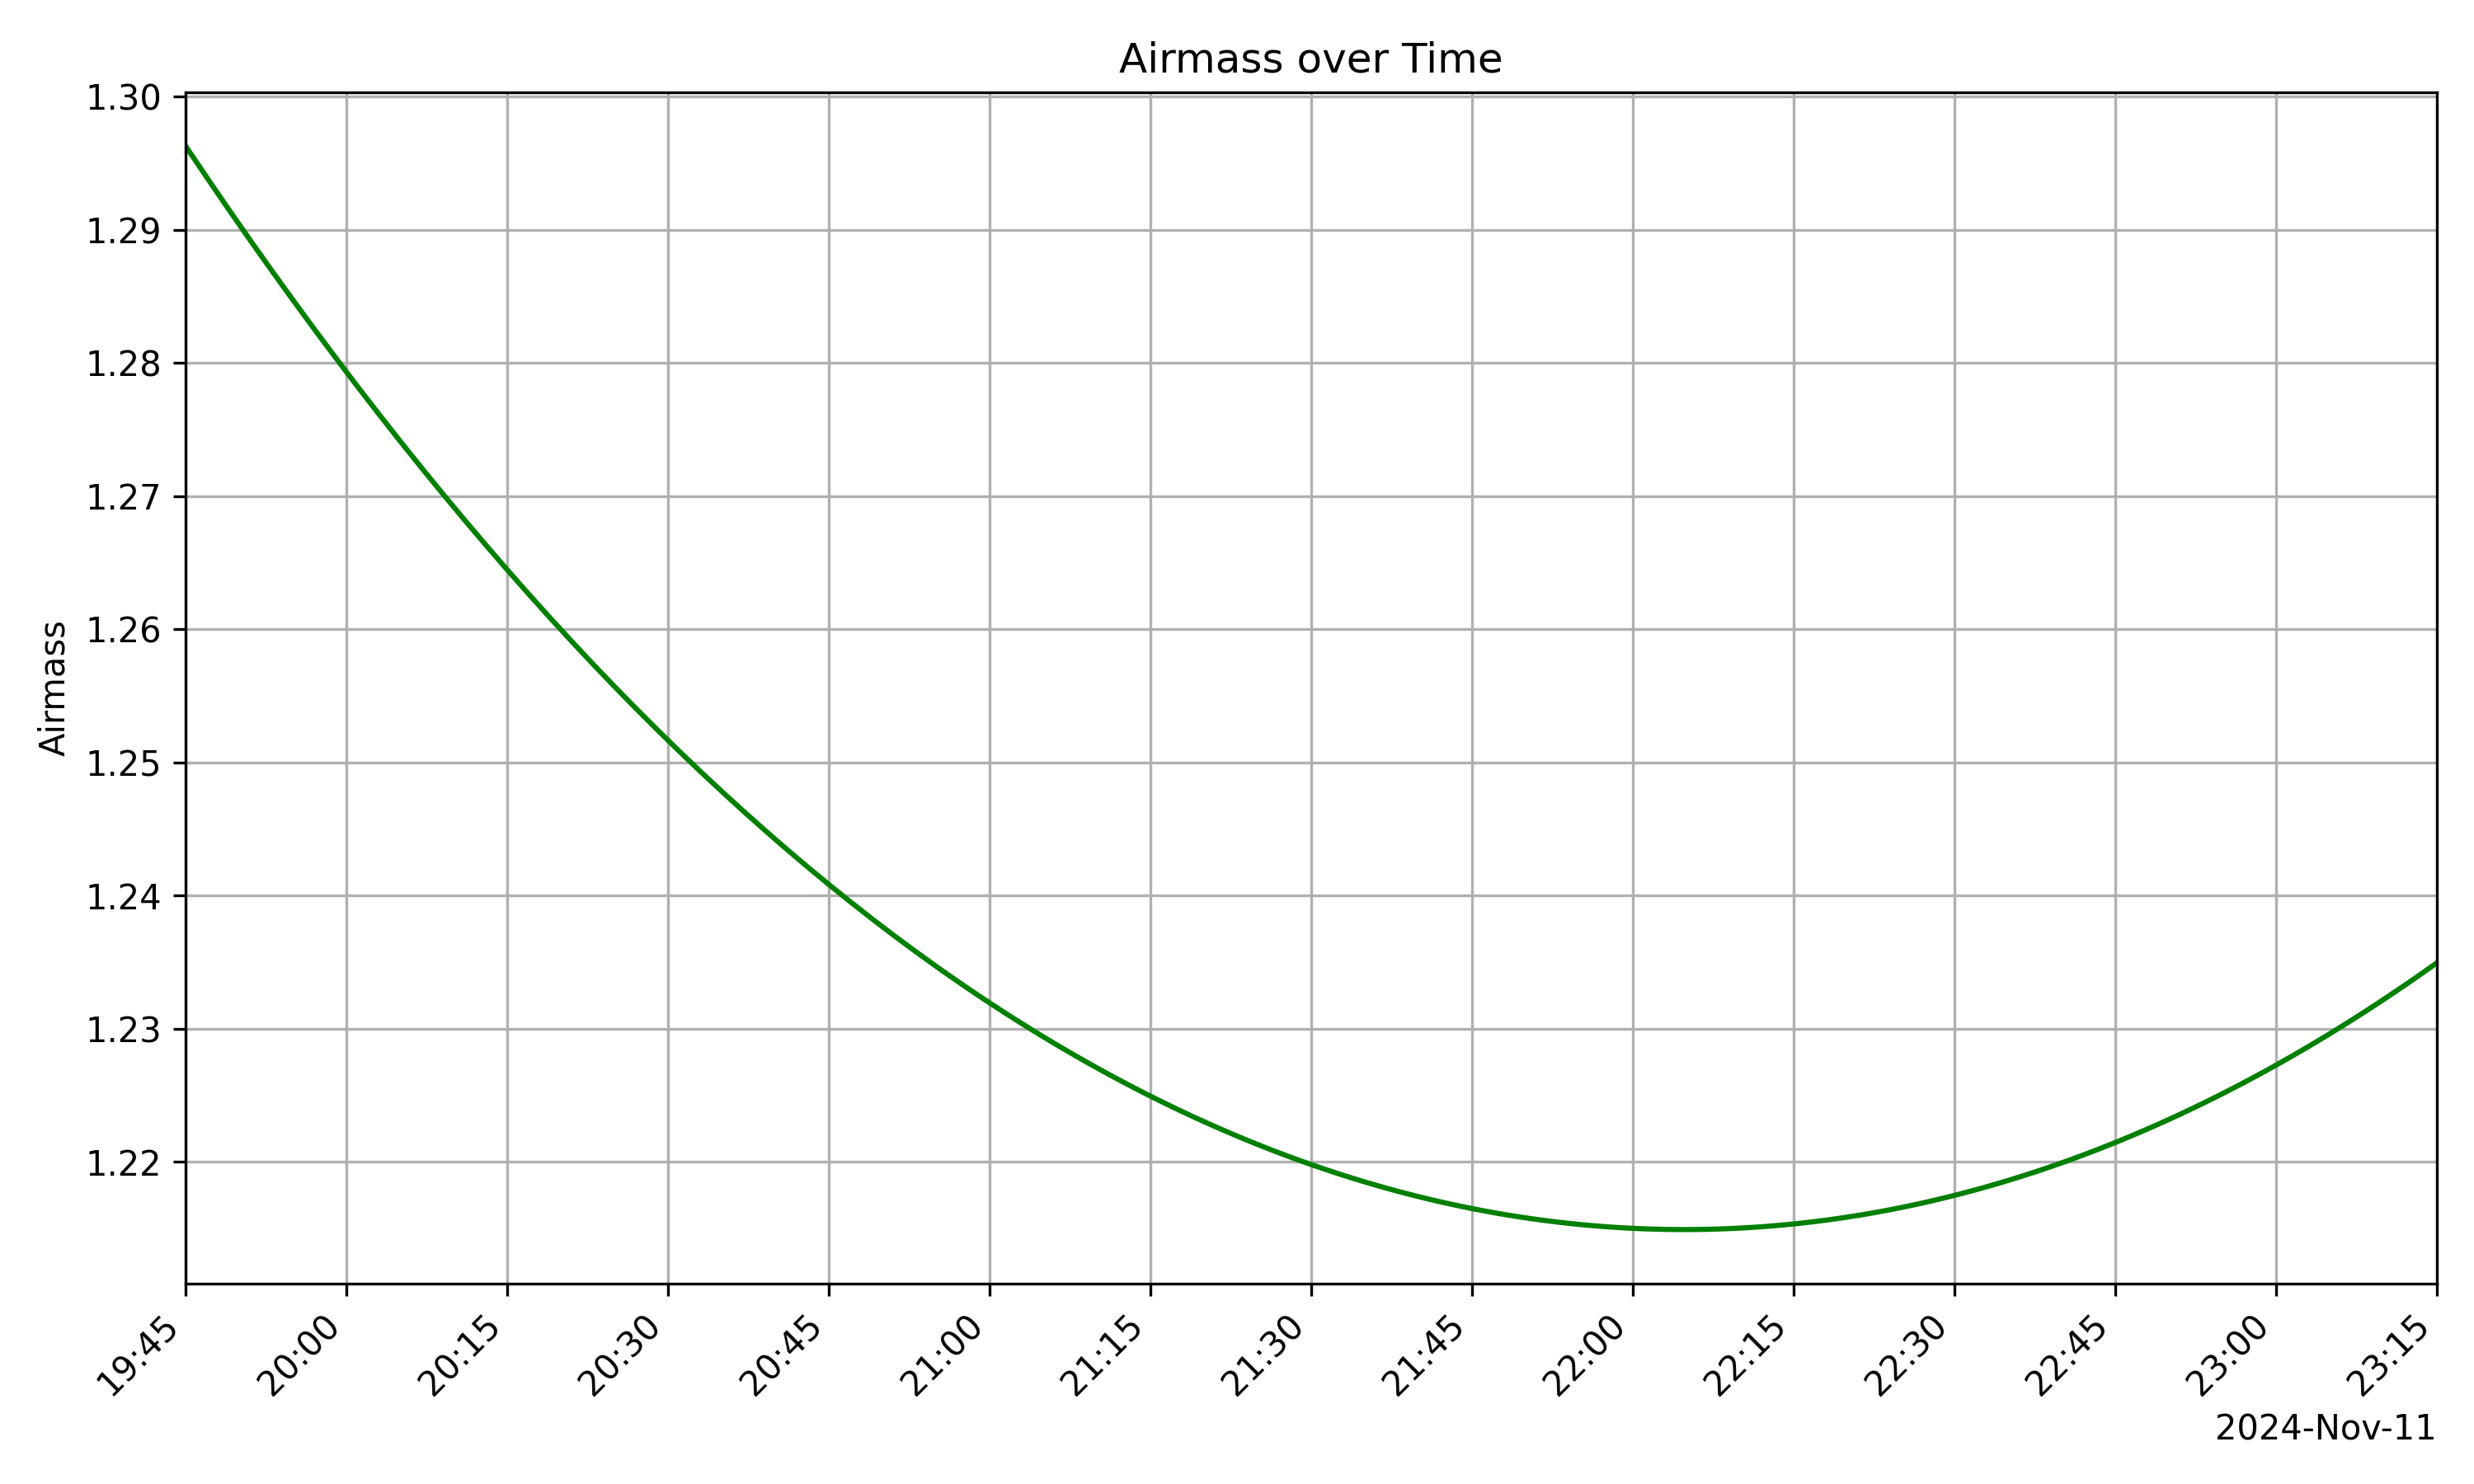
\includegraphics[width=0.9\textwidth]{./fig/airmass_over_time.png}
  \caption{エアマスの時間変化}
  \label{fig:airmass}
\end{figure}

\section{目的}
前回のレポートから, 大きく次の2つの進捗があった。
\begin{itemize}
  \item 参照星のクオリティーチェック
  \item トランジットモデルとデータの比較
\end{itemize}
それぞれについて以下で報告する。

\section{参照星のクオリティーチェック}
前回のレポートで述べた手法で参照星を選んだ。今回は, それらの参照星のクオリティーチェックを行った。
\subsection{手法}
まず, 参照星のフラックスを平均を用いて各参照星のフラックスを補正した。
その後, それぞれの参照星の等級の分散を計算した。
最後に, フラックスの変化が1\%を超えるようであれば, フラックスの変化が1\%程度の, 最低限のビンで移動平均を取った。

コードは (計算しただけであるので) 省略する。

\subsection{結果}
まず, 参照星のfinding chartを図\ref{fig:finding_chart}に示す。そして, これら参照星の等級の分散と標準偏差を表\ref{tab:compstars}に示す。

ここで, フラックス変化が$\Delta F/F$のときの等級の変化$\Delta m$は, 
$$\Delta m= -2.5\log(1+\Delta F/F)\simeq -2.5\times \dfrac{1}{\ln 10}\dfrac{\Delta F}{F}\simeq -1.09\dfrac{\Delta F}{F}$$
であるため, フラックスの変化が1\%程度であれば, 等級の変化は約0.01等級程度である。

そのため, 観測データの品質は十分であると考えられる。

\begin{figure}[H]
  \centering
  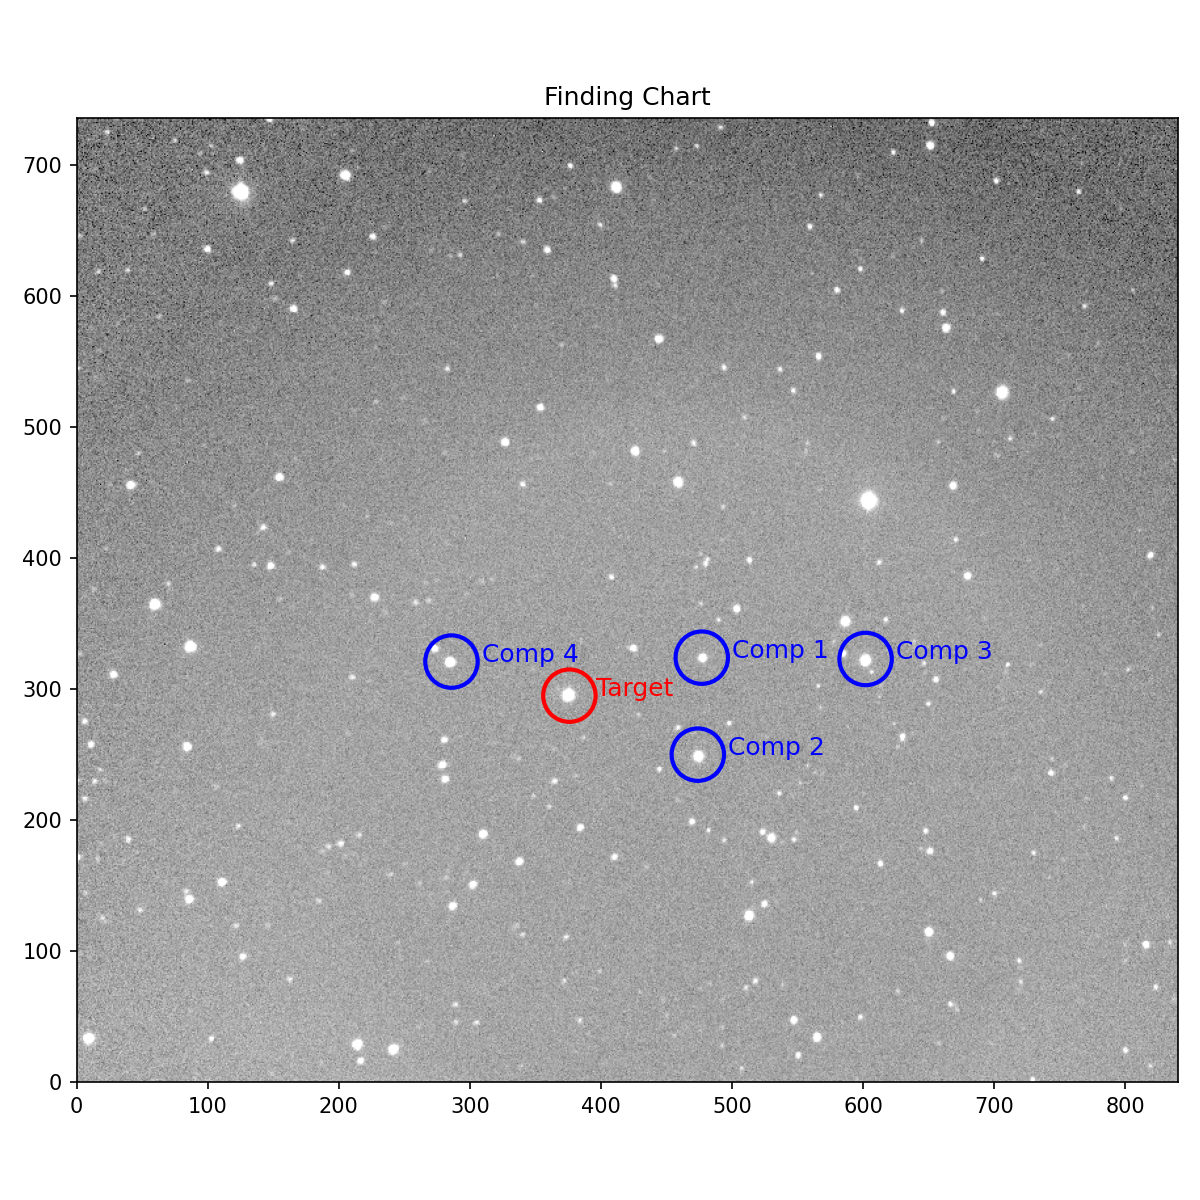
\includegraphics[width=0.65\textwidth]{./fig/finding_chart.png}
  \caption{参照星のfinding chart}
  \label{fig:finding_chart}
\end{figure}

\begin{table}[htbp]
  \centering
  \caption{参照星の分散と標準偏差}
  \label{tab:compstars}
  \begin{tabular}{c c c}
  \hline
  Comp & Variance & StdDev \\
  \hline
  1 & 0.00011 & 0.01028 \\
  2 & 0.00006 & 0.00782 \\
  3 & 0.00005 & 0.00693 \\
  4 & 0.00016 & 0.01249 \\
  \hline
  \end{tabular}
\end{table}

\section{トランジットモデルとデータの比較}
前章で品質を確認した参照星を用いて, トランジットの光度曲線を作成する。また, カタログから恒星系のパラメータを取得し, トランジットモデルを作成した。これらを重ねてプロットする。
\subsection{コード}

Python コードを掲載する。なお, パラメータは, \cite{Kabath2022}に従った。

実装の方針としては, トランジットモデルの計算の際に, トランジット中心時間をユリウス日で与え, 最後にdatetimeに変換することで, 観測データとトランジットモデルの時間を合わせた。また, 縦軸は, 観測データから補正したフラックスの, 最後の50点の中央値を1とする相対値を取った。

\subsection{結果}
図\ref{fig:transit_model}に, 光度曲線を示す。モデルの曲線が概ねデータの範囲に収まっていることが確認された。嬉しい。

\begin{figure}[H]
  \centering
  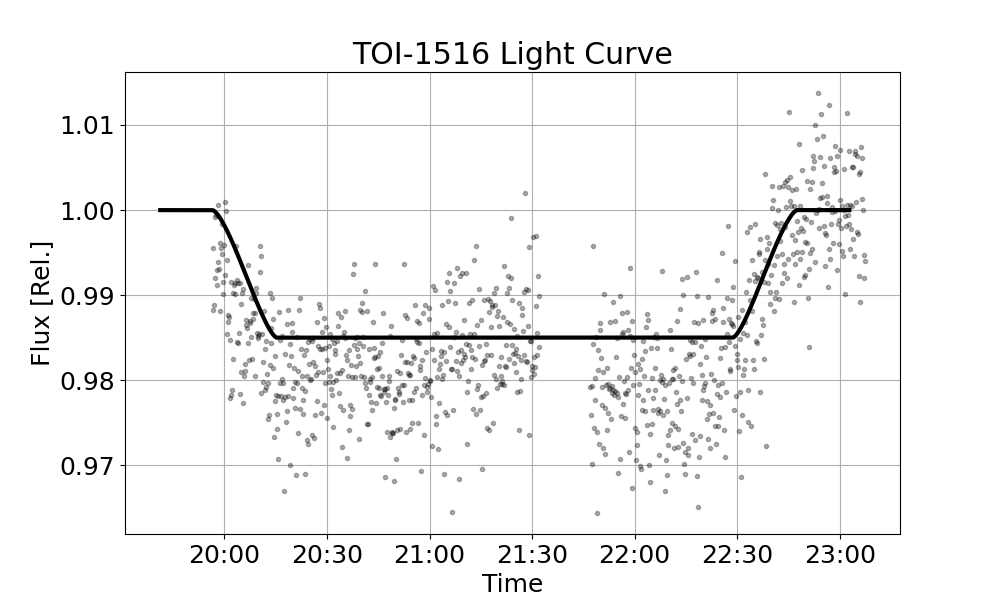
\includegraphics[width=0.9\textwidth]{./fig/light_curve_fit.png}
  \caption{TOI-1516の光度曲線}
  \label{fig:transit_model}
\end{figure}

\begin{thebibliography}{9}
\bibitem{Kabath2022}
Kabáth, P., Chaturvedi, P., et al.\ 
2022, 
\textit{Monthly Notices of the Royal Astronomical Society}, 
513(4), 5955--5972.
\end{thebibliography}
\end{document}